% Common use
\psfrag{c1}[c][c] {$\Bd_{G_{i}}$}
% \psfrag{c2}[c][c] {$\Bd_{E}$}
\psfrag{c2}[c][c] {$V_{e}$}
\psfrag{as}[c][c]   {\scriptsize $a^{\!\ast}$}
\psfrag{xb}[c][c] {$\Bx \in \Omega$}
\psfrag{concen}[c][c] {$\textsc{structure tensor } \BM^{R} \circ \BM^{E}$}
\psfrag{cbar}[c][c] {$\phi=\bar{\phi}$}
\psfrag{dbh}[c][c] {$\partial\Omega^{h}_{N}$}
\psfrag{dbc}[c][c] {$\partial\Omega^{\phi}$}

% Cation field
\psfrag{dispca}[c][c]  {\scriptsize $\textsc{Cation } \text{Li}^{+}
		\textsc{ field }  c^{p}$}
\psfrag{cp}[c][c]  {$c^{p}$}

% Anion field
\psfrag{dispan}[c][c] {\scriptsize $\textsc{Anion field } c^{m}$}
\psfrag{cm}[c][c]  {$c^{m}$}

% Vacancy field
\psfrag{dispva}[c][c]   {\scriptsize $\textsc{Vacancy field } c^{n}$}
\psfrag{cn}[c][c]  {$c^{n}$}

% Displacement field
\psfrag{disp}[c][c] {\scriptsize $\textsc{displ. field } \Bu$}
\psfrag{ud}[c][c]   {$\Bu$}
\psfrag{pbar}[c][c] {$\Bu=\bar{\Bu}$}
\psfrag{dbt}[c][c]  {$\partial\Omega^{\Bt}_{N}$}
\psfrag{dbphi}[c][c]{$\partial\Omega^{\Bu}_{D}$}
\psfrag{n}[c][c]    {$\Bn$}
\psfrag{tbar}[c][c] {$\Bsigma\cdot\Bn = \bar{\Bt}$}

% Temperature field
\psfrag{temp}[c][c]  {\tiny $\textsc{Temp. field } \theta$}
\psfrag{te}[c][c]    {$\theta$}
\psfrag{tebar}[c][c] {$\theta = \bar{\theta}$}
\psfrag{dbte}[c][c]  {$\partial\Omega^{\theta}_{D}$}
\psfrag{hbar}[c][c]  {$\Bq\cdot\Bn = \bar{h}$}

% Space charge layer
\psfrag{istb}[c][c] {\tiny $\textsc{scl}$}
\psfrag{itf}[c][c]  {\scalebox{0.25}{$\textsc{(SE$|$SSE)-Interface}$}}
\psfrag{intf}[c][c] {\tiny $\textsc{Dendrite growth}$}

% Nucleation
\psfrag{gfcr}[c][c] {\tiny $\textsc{Griffith criterion } a^{\!\ast}$}
\psfrag{nclp}[c][c] {\tiny $\textsc{Cracking nucleation}$}
\psfrag{nctp}[c][c] {\tiny $\textsc{Nucleation tip}$}
\psfrag{ncpt}[c][c] {\tiny $\textsc{Nucleation point}$}
\psfrag{nczn}[c][c] {\tiny $\textsc{Nucleation zone}$}
\psfrag{agrf}[c][c] {\tiny $a^{\!\ast}\!\!=\!a_{\text{Griffith}}$}

% Misorientation
\psfrag{misso}[c][c] {\scriptsize $\textsc{Electrostatic}\, V_{e}$}
\psfrag{po}[c][c] {\scriptsize $\textsc{potential}\, V_{e}$}
% \psfrag{misso}[c][c] {\scriptsize $\textsc{Misorientation } \BM = \Bd \otimes \Bd $}
\psfrag{gbl}[c][c] {\tiny $\textsc{Global direction: Uniform electric field } \Bd_{E}$}
\psfrag{lcl}[c][c] {\tiny $\textsc{Local direction:  Crystallographical orientation } \Bd_{G_{i}}$}
\psfrag{lcd}[c][c] {\tiny $\textsc{Local direction}$}
\psfrag{gbd}[c][c] {\tiny $\textsc{Global direction}$}
\psfrag{pl}[l][l] {\tiny $+$}
\psfrag{mn}[l][l] {\tiny $-$}
\psfrag{c1m}[c][c] {\tiny $\Bd_{G_{i}}$}
\psfrag{c2m}[c][c] {\tiny $\Bd_{E}$}
\psfrag{str}[c][c] {$\BM^{R} := \Bd^{R} \otimes \Bd^{R}$}
\psfrag{mde}[c][c] {$\BM^{E} := \Bd^{E} \otimes \Bd^{E}$}

% Boundary condition
\psfrag{bdc}[c][c] {\scriptsize $\textsc{Boundary condition around pre-existing crevice open at (SE$|$SSE)-Interface}$}

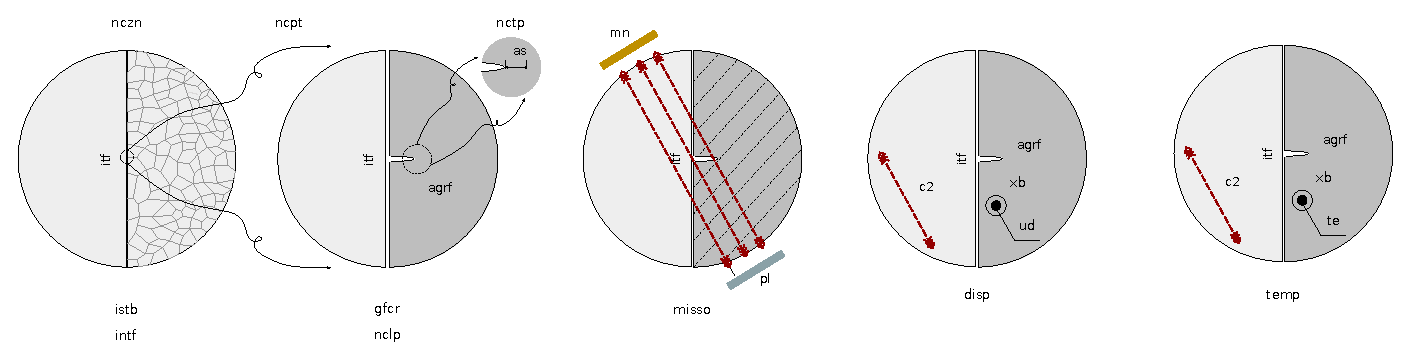
\includegraphics[width=0.85\textwidth]{structuralfivefields_multi_edited.eps}